\section{Methods}

In order to demonstrate that the DISHTINY platform selects for detectable hierarchical transitions in individuality, we performed experiments where cell-like organisms evolved parameters to control manually designed behaviors such as resource-sharing, reproductive decision-making, and apoptosis.
We will first cover the design of the DISHTINY platform and then describe the simple cell-like organisms we used to evaluate the platform.

\subsection{DISHTINY}

\begin{figure*}[t]
\begin{center}
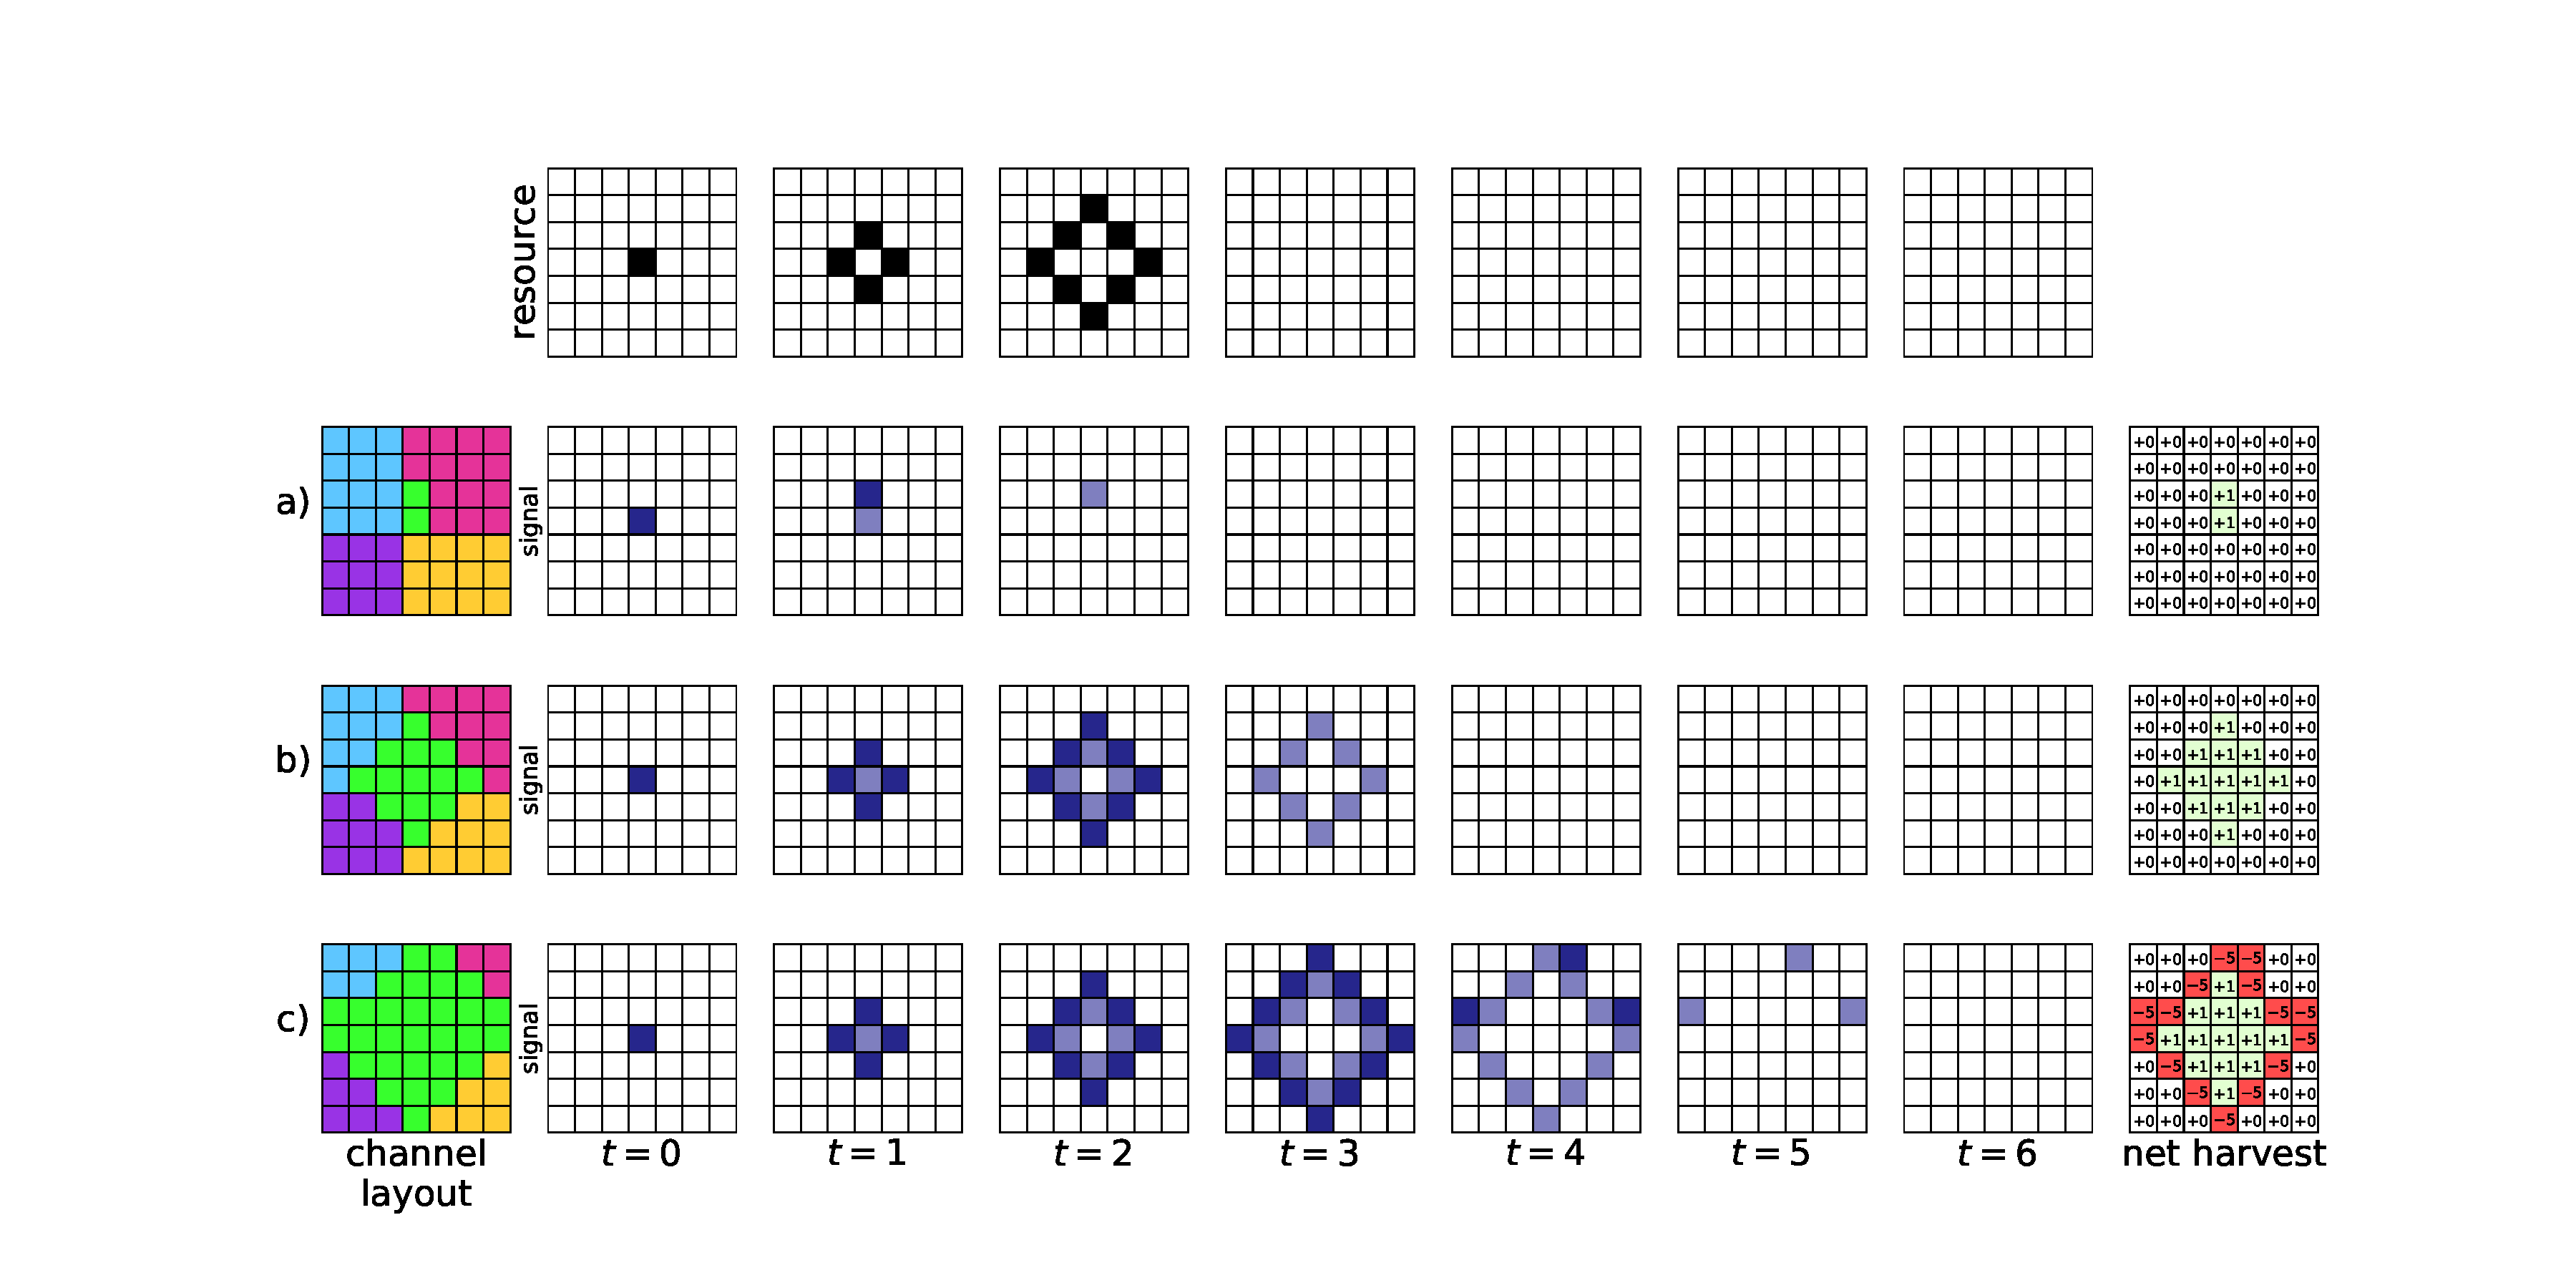
\includegraphics[width=2.0\columnwidth]{img/explanatory}
\caption{
\textbf{Activation signaling, and net resource collection for three different channel configurations during a resource wave event.}
At the top, a resource wave is depicted propagating over three updates and then ceasing for four updates (left to right).
In row $a$, a small channel-signaling group (far left, in green) is activated; tracking the resource wave (top) yields a small net resource harvest (far right).
In row $b$, an intermediate-sized channel-signaling group yields a high net resource harvest.
Finally, in row $c$, a large channel-signaling group incurs a net negative resource harvest.
In rows $a$, $b$, and $c$, dark purple indicates the active state, light purple indicates the quiescent state, and white indicates the ready state.
}
\label{fig:explanatory}
\end{center}
\end{figure*}


DISHTINY allows cell-like organisms to replicate across a toroidal grid.  As cells reproduce, they can optionally share signaling channels with their offspring.
Over discrete timesteps (``updates''), the cells can collect a continuous-valued resource, either hoarding it or sharing it with others on a signaling channel.
Once sufficient resource has been accrued, cells may pay $8.0$ resource to place a daughter cell on an adjoining tile of the toroidal grid (i.e., reproduce), replacing any existing cell already there.

As shown at the top of Figure \ref{fig:explanatory}, resources appear at a single point and spread in diamond-shaped waves.
Each update the resource wave advances one grid tile outward, disappearing when it reaches a predefined limit.
Cells must be in a costly ``activated'' state to collect resource as it passes.
The cell at the starting position of a resource wave is automatically activated, and will send the activate signal to neighboring cells on the same signaling channel.
The newly activated cells, in turn, activate their own neighbors registered to the same signaling channel.
Neighbors registered to other signaling channels do not activate.
Each cell, after sending the activation signal, enters a temporary quiescent state so as not to reactivate from the signal.
In this manner, cells sharing a signaling channel activate in concert with the expanding resource wave.
As shown Figure \ref{fig:explanatory}$a,b$, the rate of resource collection for a cell is determined by the size and shape of of its same-channel signaling network;
small or fragmented same-channel signaling networks will frequently miss out on resource as it passes by.

Each cell pays a resource cost when it activates.
This cost is outweighed by the resource collected such that cells that activate in concert with a resource wave derive a net benefit.
Recall, though, that resource waves have a limited extent.
Cells that activate outside the extent of a resource wave or activate out of sync with the resource wave (due to an indirect path from the cell that originated the signal) pay the activation cost but collect no resource.
Cells that frequently activate erroneously use up their resource and die.
In our implementation, organisms that accrue a resource debt of $-11$ or greater are killed.
This scenario is depicted in Figure \ref{fig:explanatory}$c$.

In this manner, ``Goldilocks'' --- not to small and not too big --- signaling networks are selected for.
Based on a randomly chosen starting location, resource wave starting points (seeds) are tiled over the toroidal grid such that the extents of the resource waves touch, but do not overlap.
All waves start and proceed synchronously;
when they complete, the next resource waves are seeded.
This process ensures that selection for ``Goldilocks'' same-channel signaling networks is uniformly distributed over the toroidal grid.

Cells control the size and shape of their same-channel signaling group through strategic reproduction.
Three choices are afforded: whether to reproduce at all, where among the four adjoining tiles of the toroidal grid to place their offspring, and whether the offspring should be registered to the parent's signaling channel or be given a random channel ID (in the range 1 to $2^{22}$).
No guarantees are made about the uniqueness of a newly-generated channel ID, but chance collisions are rare.

% @CAO: HERE is where we first introduce how multiple channels work; only from here on do we need to worry about talking about "same-channel signaling"
% @MAM: I think there is some confusion about channel vs. level...
Hierarchical levels are introduced into the system through multiple separate, but overlaid, instantiations of this resource wave/channel-signaling scheme.
We refer to each independent resource wave/channel-signaling system as a ``level.''
In our experiments, we allowed two resource wave/channel-signaling levels, identified here as level one and level two.
On level one, resource waves extended a radius of three toroidal tiles.
On level two they extended a radius of 24 toroidal tiles.
On both levels, activated cells netted $+1.0$ resource from a resource wave, but suffered an activation penalty of $-5.0$ if no resource was available.
Due to the different radii of resource waves on different levels, level one selects for small same-channel signaling networks and level two selects for large same-channel signaling networks.

Cells were marked with two separate channel IDs, one for level one and another for level two.
We enforced hierarchical nesting of same-channel signaling networks during reproduction:
daughter cells may inherit neither channel ID, just the level-two channel ID, or both channel IDs.
Daughter cells may not inherit only the level-one channel ID while having a different level-two channel ID.
The distribution of IDs across the level-two and level-one channels can be envisioned by analogy to political countries and territories.
Each country (i.e., level-two channel network) may have one or many territories (i.e., level-one channel network).
However, no territory spans more than one country.
Figure \ref{fig:outcome_grids} depicts hierarchically nested channel states at the end of three evolutionary runs.

Channel IDs enable straightforward detection of an evolutionary transition in individuality.
Because common channel IDs may only arise systematically through inheritance, common channel IDs indicate a close hereditary relationship in addition to a close cooperative relationship.
Because new channel IDs arise first in a single cell, same-channel signaling networks are reproductively bottlenecked, ensuring meaningful reproductive lineages at the level of the same-channel signaling network.
To recognize an evolutionary transition in individuality, we therefore evaluate
\begin{enumerate}
\item Do cells with the same channel ID choose to share resources (e.g., cooperate)?
\item Is there division of reproductive labor between members of the same channel (e.g., do cells at the interior of a network cede reproduction to those at the periphery?)
\end{enumerate}
If these conditions are met among cells sharing the same level-one channel, we can conclude that a first-level transition in individuality has occurred.
Likewise, if these conditions are met among cells sharing the same level-two channel, we can conclude that a second-level transition in individuality has occurred.

\subsection{Organisms}

We performed our experiments using cell-like organisms composed of 15 floating-point parameters, each controlling a specific strategy component pertinent to transitions in individuality (i.e., reproductive division of labor, resource pooling, apoptosis, propagule generation, and propagule endowment).
These particular cell-like organisms are in no way inherent to the DISHTINY platform, but were merely developed to study transitions using as simple a models system as feasible.
On reproduction, we applied mutation to each parameter independently with probability $0.00005$.

The \textbf{aversion parameters} ($\bm{A_1}$ and $\bm{A_2}$) allow cells to avoid reproducing over neighbors sharing the same signaling channel.
Specifically, they control the probability that a cell declines to supplant a neighbor sharing the same level-one ($A_1$) or level-two ($A_2$) channel ID.
If a cell declines to place its offspring in all four adjoining tiles, it decides not to reproduce.
Mutation is performed by a redraw from the uniform distribution $U(-0.5,1.5)$ clamped to the range $[0,1]$.

The \textbf{resource allocation parameters} control the proportion of resources that go to the cell's stockpile ({$\bm{P_{c}}$), its level-one channel's resource pool ($\bm{P_1}$), or its level-two channel's resource pool ($\bm{P_2}$).
These parameters are initialized by a draw from $U(-1.0, 2.0)$ clamped to the range $[0,1]$ and mutated by addition of a normal value drawn from $N(0.0,0.2)$ with the result clamped to the range $[0,1]$.
The set $P_{c}, P_1, P_2$ is always normalized to sum to 1.

Channel resource pools are identical to an organism's individual stockpile, except that any deficit is distributed evenly among the individual organism's stockpile.
On every update, cells can spend from their individual stockpile to reproduce or from a channel pool, with priority given to cells nearest to the centroid of that pool's members.
As such, pool-funded reproduction fills in a same-channel signaling network from the inside out and help produce diamond-shaped same-channel signaling networks.
(Distance is measured using the taxicab metric.)

\textbf{Channel cap parameters} $\bm{C_1}$ and $\bm{C_2}$ regulate the size of same-channel signaling networks.
When an organism reproduces, it checks the size of its level-one signaling network against $C_1$ and the size of its level-two signaling group against $C_2$.
If neither cap is met or exceeded, then the organism will produce an offspring sharing both of its channel IDs.
If only the $C_1$ cap is exceeded, then the organism will produce an offspring with new level-one channel ID but identical level-two channel ID.
Finally, if the $C_2$ cap is exceeded, then the organism will produce an offspring with new IDs for both channels.
For level 1 caps, these parameters are initialized by a draw from $U(0.0, 16.0)$.
For level 2 caps, these parameters are initialized by a draw from $U(0.0, 128.0)$.
Both are mutated by addition of a value drawn from $N(0.0,24.0)$ with the result clamped to be non-negative.

The \textbf{endowment parameters} $\bm{E_{c}}$, $\bm{E_1}$, and $\bm{E_2}$ determine the amount of resource provided to offspring.
This endowment is paid as an additional cost by the cell stockpile (or same-channel resource pool) funding a reproduction.
The full amount of the received endowment is divided between the daughter cell's stockpile, level-one same-channel resource pool, and level-two same-channel resource pool according to the offspring's resource allocation parameters.
$\bm{E_{c}}$ is the endowment amount paid to an offspring that shares both channel IDs of the parent;
$\bm{E_1}$ is the endowment paid to an offspring that shares just the level-two channel ID of the parent;
and $\bm{E_2}$ is the endowment paid to an offspring that shares neither the level-one nor level-two channel ID of the parent.
Endowed resources help new-channel propagules to rapidly grow their signaling network in order to begin collecting resource at a rate competitive to other well-established same-channel signaling networks.
In order to provide that adequate resource remained to ensure parental stability, endowment was paid out only after twice the endowment amount had been accrued (leaving an amount of resource equal to the endowment remaining with the parent).
Cell level endowments are initialized by a draw from $U(0.0, 5.0)$.
Level-one endowments are initialized by a draw from $U(0.0, 80.0)$.
Level-two endowments are initialized by a draw from $U(0.0,405.0)$.
All endowments are mutated by addition of a value drawn from $N(0.0,10.0)$ with the result clamped to be non-negative

Parameters $\bm{M_{c}}$, $\bm{M_1}$, and $\bm{M_2}$ control the \textbf{apoptosis response to mutation}.
Each time that a mutation occurs during reproduction, the mutated offspring attempts suicide with probability $M_{c}$ if it shares both channel IDs of its parent, probability $M_1$ if it shares just the level-two channel ID of its parent, and probability $M_2$ if it shares neither channel ID of the parent.
The $M_x$ value applied is from the offspring's genotype after mutation.
Attempted suicide succeeds 90\% of the time.
This capacity enables first- or second-level individuals to combat somatic mutation.
Initialization and mutation each of these parameters is performed by a redraw from the distribution $U(-0.5,1.5)$ clamped to the range $[0,1]$.

Finally, parameters $\bm{S_1}$ and $\bm{S_2}$ \textbf{fine-tune site choice for offspring placement}.
If an organism is placing an offspring with identical channel IDs, with probability $S_1$ the four possible sites for offspring placement are considered in order of increasing distance from the centroid of the parent's level-one signaling network.
If an organism is placing an offspring with identical level-two channel ID but different level-one channel ID, with probability $S_2$ the four possible sites for offspring placement are considered in order of increasing distance from the centroid of the parent's level-two same-channel signaling network.
Otherwise, the four possible sites for offspring placement are considered in a random order.
Initialization and mutation are performed by a draw from the distribution $U(-0.5,1.5)$ clamped to the range $[0,1]$.

\subsection{Experiments}

We performed experiments to assess the evolutionary trajectories of populations in DISHTINY.
We seeded each tile on the $120 \times 120$ toroidal grid with a randomized organism and ran the simulation for 20 million updates.
In order to facilitate turnover, we culled the population intermittently.
Starting at update 500,000, and every 50,000 updates thereafter, we randomly selected Level 2 channel IDs and killed all cells with that channel ID, continuing until at least 5\% of grid tiles were empty.
We performed 50 replicates within this treatment.
On average, each cellular generation took just over 500 updates.
Across all successive 10,000 update segments of all replicates, the mean number of cellular generations elapsed per 10,000 updates was 19.2 with a standard deviation of 2.7 cellular generations per 10,000 updates.

In order to detangle the impact of same-channel signaling networks with respect to kin recognition and with respect to cooperation to increase resource collection rate, we performed control evolutionary trials where same-channel signaling networks did not improve cellular resource collection rate.
Under control conditions, same-channel signaling networks just helped cells recognize other related cells.
In our implementation, this treatment corresponded to resource waves with radius 1 (i.e., the resource wave did not expand beyond its seed) that paid out 1.0 resource unit to cells and zero cost for erroneous activation.
All other aspects of control runs, including the functionality of all lifestyle parameters, were otherwise identical to standard conditions.
We performed 50 replications of the control treatment.
In control runs, generations progressed much faster, taking only around 50 updates.
Across all successive 10,000 update segments of all replicates, the mean number of cellular generations elapsed per 10,000 updates was 211.1 with a standard deviation of 43.8 cellular generations per 10,000 updates.
Higher resource inflow rate under the control conditions likely contributed the faster cellular generation rate compared to the control conditions.

In standard evolutionary runs, we observed a spectrum of evolved resource-caching strategies.
To assess the relative fitness of these evolved organisms, we ran competitions between the most common genotype from three standard evolutionary runs.
The first genotype allocated resource exclusively to its first-level same-channel resource pool (i.e., $P_{1} = 1.0$), the second split resource evenly between its first-level and second-level resource pool (i.e., $P_{1} = P_{2} = 0.5$), and the third allocated resource primarily to the second-level resource pool (i.e., $P_{2} > P_{1}$).
(No most-common genotypes allocated resource exclusively to the second-level resource pool).
We seeded each competition with three copies of each genotype, uniformly spaced over the $120 \times 120$ toroidal grid with random arrangement.
Each competition lasted 2 million updates.
We performed 50 runs in this experiment.

\subsection{Implementation}

We implemented our experimental system using the Empirical library for scientific software development in C++, available at \url{https://github.com/devosoft/Empirical}.

We performed our computational experiments at the Michigan State University High Performance Computing Center.
Unfortunately, concurrent efforts to prepare the system for an operating system upgrade caused intermittent disk unavailability and checkpoint-restart failure.
By cursory inspection of the line count of our most intensively written data files we estimate that 5-10\% of content is missing.
Lines appear to be missing in contiguous sections (corresponding to contiguous update ranges).
Except where explicitly noted, missing data is not relevant to our analyses and visualizations, which primarily describe end-states where data from all runs is available.
Due to checkpoint-restart failures, we curtailed our standard-condition evolutionary runs from a planned 25M to 20M updates and our control evolutionary runs to 250k updates.

Each replicate of standard evolutionary experiments required approximately six days of compute time to reach 20 million updates.
Each replicate of control evolutionary experiments expended on the order of one day of compute time to reach 250 thousand updates.
Control runs were slower than standard runs, likely due to a higher per-update cellular generation rate.
Each replicate of competition experiments consumed approximately ten hours of compute time.
For standard evolutionary experiments, data processing required approximately four hours of compute time per run.
Other data processing was computationally negligible.

The code used to perform and analyze our experiments, our figures, data from our experiments, and a live in-browser demo of our system is available via the Open Science Framework at \url{https://osf.io/ewvg8/}.
